%%%%%%%%%% PREAMBLE %%%%%%%%%%

%MNRAS style
\documentclass[fleq,usenatbib]{mnras}
%default MNRAS packages
\usepackage{newtxtext,newtxmath}
\usepackage[T1]{fontenc}
\usepackage{ae,aecompl}
\usepackage{color,soul}
% user packages
\usepackage{graphicx}
\usepackage{amsmath}
\usepackage{amssymb}
\usepackage{dsfont}
%user commands
\newcommand{\acro}{TREVR}
\providecommand{\e}[1]{\ensuremath{\times10^{#1}}}
\newcommand{\bigO}[1]{\mathcal{O}\left(#1\right)}
\newcommand{\NS}{N_{\rm source}}
\newcommand{\NR}{N_{\rm ray}}
%%%%%%%%%%%%%%%%%%%%%%%%%%%%%%

%%%%%%%%%% TITLE PAGE %%%%%%%%%%

\title[]{\acro{}: A general $\bigO{N\log^2N}$ radiative transfer algorithm}

\author[J. J. Grond et al.]{
J. J. Grond,
R. M. Woods,
J. Wadsley \thanks{E-mail:  wadsley@mcmaster.ca}
and H. M. P. Couchman
\\
Department of Physics and Astronomy, McMaster University, Hamilton, Ontario L8S
 4M1, Canada}

\date{Accepted XXX. Received YYY; in original form ZZZ}

\pubyear{2018}

\begin{document}
\label{firstpage}
\pagerange{\pageref{firstpage}--\pageref{lastpage}}
\maketitle

% abstract of the paper
\begin{abstract}
We present \acro{} (Tree-based Reverse Ray Tracing), a general algorithm for 
computing the radiation field in astrophysical simulations. \acro{} 
prioritizes the ability to handle large numbers of sources and computational 
speed whilst maintaining a specified level of accuracy via adaptive 
refinement. \acro{} is based on a \emph{tree} data structure similar to many 
gravity and hydrodynamics solvers. This allows for computation of the 
radiation field in $\mathcal{O}(N \log \NS)$ time without 
absorption and $\mathcal{O}(N \log \NS \log{N})$ time with 
absorption. This impressive  scaling is made possible by merging sources of 
radiation according to an opening angle criteria and walking the tree 
structure to trace a ray. The computational complexity we quote accounts for 
the use of adaptive refinement, a main feature that is unique to \acro{} among 
other radiative transfer methods. We provide a suite of tests demonstrating 
the algorithm's ability to accurately compute fluxes, ionization fronts and 
shadows. We also analyze the algorithm's computational complexity, in how it 
scales with the number of sources and sinks. Further examinations of how the 
aforementioned refinement criterion's value affects computational cost and 
accuracy are presented. Finally, we discuss strengths and shortcomings of this 
algorithm, how they constrain the types of problems \acro{} can handle and how 
these shortcomings can be remedied if possible.

\end{abstract}

% Select between one and six entries from the list of approved keywords.
% Don't make up new ones.
\begin{keywords}
radiative transfer -- methods: numerical
\end{keywords}

%%%%%%%%%%%%%%%%%%%%%%%%%%%%%%

%%%%%%%%%% BODY OF PAPER %%%%%%%%%%

\section{INTRODUCTION}\label{sec:intr}
Radiation is arguably the most important physical phenomena to the field of
astrophysics. Almost all of the information we receive from outer space comes 
in the form of photons we detect on or around earth. Understanding the process 
of radiative transfer (RT) is key in interpreting this information, as the 
photons are affected by the medium they travel through on their way to our 
telescopes and detectors. Interactions between photons and the medium do not 
only affect the photons themselves but the matter as well. Photons and baryons 
exchange energy and momentum, affect the excitation and ionization states of 
said baryons and thus determine the chemical and thermodynamic properties of 
the bulk medium. This in turn makes radiation a driving factor in many of the 
physical processes we study.

On galaxy scales, the question of how feedback mechanisms affect star and 
galaxy formation is one of these physical processes we can study. Stellar 
feedback comes in the form of photoionization by ultraviolet (UV) radiation, 
stellar winds and supernovae (cite here), the latter of which has been 
a main focus in simulations in previous years (cite a bunch of SN feedback 
papers?). It is important to note that even though supernovae might be 
spectacularly powerful events, ionizing radiative output from stellar 
populations in the UV regime contribute two orders of magnitude more power at 
early times and about 50 times more energy over the course of a stellar 
population's lifetime. This is made evident in Fig. \ref{fig:uvsn}, a 
plot of luminosity output per solar mass as a function of time from stellar 
populations created via output from the stellar evolution code Starburst99 
\citep{leithererEt99}. 
\begin{figure}
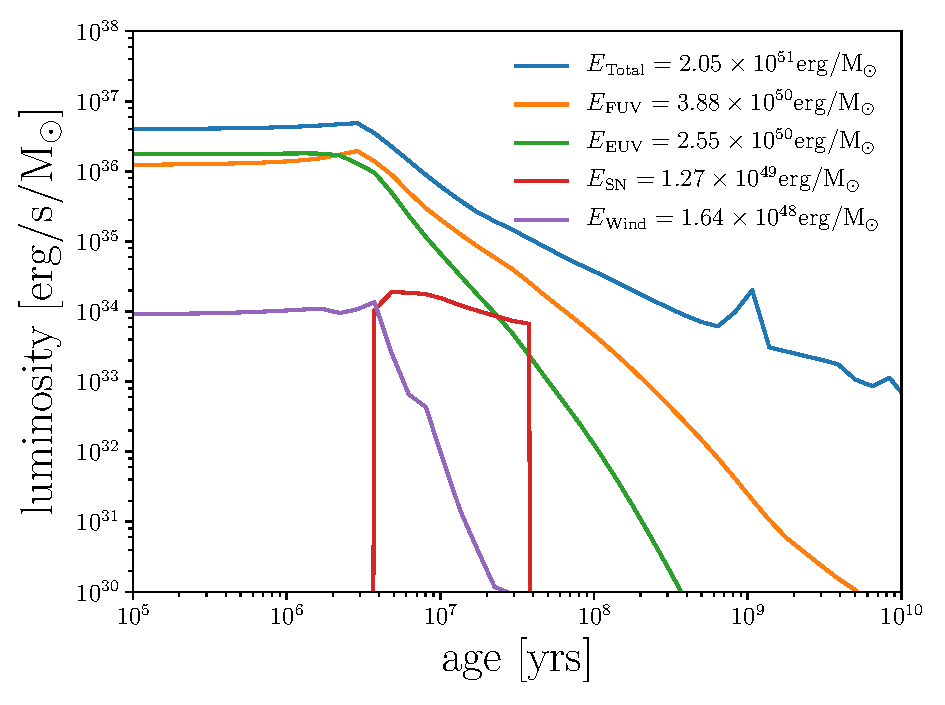
\includegraphics[width=1\linewidth]{Figures/uvsn.pdf}
\caption{Luminosity per solar mass as a function of time for a stellar 
population having a Chabrier initial mass function \citep{chabrier03}.}
\label{fig:uvsn}
\end{figure}
However, the way in which this massive output of UV radiation is deposited 
and consequently affects the interstellar medium (ISM) is still unclear 
(cite... from fervent paper - conflicting results from Murray 2011, Dale 
et al. 2012, Faucher-Gigu`ere et al. 2013, Hopkins et al. 2014).

With such a large amount of energy input from stellar sources and questions 
still left open about how it affects the ISM, it may then come as a surprise 
that RT has historically been treated rather poorly in most large scale 
astrophysical simulations, usually as some imposed uniform background. This is 
not because of carelessness or lack of effort, but because RT is intrinsically 
a complicated problem. The complexity of this problem is evident in the 
classical RT equation \citep[e.g.][]{mihalasMihalas84},
\begin{equation} \label{eq:classicrt}
\left[ \frac{1}{c} \frac{\partial}{\partial t} + \mathbf{\hat{n} \cdot \nabla}
 \right] I\left(\mathbf{x}, \mathbf{\hat{n}}, t, \nu\right) = 
\epsilon\left(\mathbf{x}, \mathbf{\hat{n}}, t, \nu\right) - 
\alpha\left(\mathbf{x}, \mathbf{\hat{n}}, t, \nu\right) 
I\left(\mathbf{x}, \mathbf{\hat{n}}, t, \nu\right),
\end{equation} 
where $I$, $\epsilon$ and $\alpha$ are the intensity, emissivity and 
extinction coefficients respectively and all depend on position $\mathbf{x}$, 
unit direction of light propagation $\mathbf{\hat{n}}$, time $t$ and frequency 
$\nu$. Apart from being a seven dimensional problem, RT has a high 
characteristic speed of $c$, the speed of light. Also, unlike a force at a 
distance problem such as gravity, RT depends on the properties of the 
intervening material which is handled by the extinction coefficient $\alpha$.

Because of this complexity, a naive numerical solution to the RT problem 
scales with the number of resolution elements like $\bigO{N^{7/3}}$. This 
costly scaling is simply a result of the three major parts that go into 
computing the radiation field in a simulation. Firstly, a radiation field is 
represented by a simulation's $N$ resolution elements, so the field intensity 
needs to be computed at $N$ points in the simulation volume. Secondly, each 
resolution element's intensity value is made up of contributions from $\NS$ 
sources of radiation. This can also be thought of as $\NS$ rays of light being 
computed per resolution element. This leads to an already nasty scaling for 
the total number of rays computed in a simulation going as $\NR = N 
\times \NS$, which is like $\bigO{N^2}$ assuming the $\NS = N$. This fact 
alone limits rudimentary RT methods to only small scale problems 
(such as...?), where the number of sources is only a handful, to avoid 
$\bigO{N^2}$ scaling. Finally, each ray of light interacts with the medium 
along its path as mentioned earlier. Since the medium is represented by the 
simulation's $N$ resolution elements and $N$ is proportional to the simulation 
volume, a one dimensional ray intersects with $\bigO{N^{1/3}}$ resolution 
elements. Using the total number of resolution elements interacted with as a 
measure of computational cost we get that the computational cost is 
proportional to $N \times \NS \times N^{1/3}$, which is like $\bigO{N^{7/3}}$. 
This poor scaling with resolution elements makes it unfeasible to simulate RT 
along with gravity and hydrodynamics methods that scale like $\bigO{N\log N}$. 
After breaking down the source of computational complexity in the RT problem 
it is evident that something needs to be done about the strong dependence on 
$\NS$ and the $N^{1/3}$ cost of computing each ray to attain a feasible RT 
method.

To avoid the intrinsic complexity of the RT problem, a feasible method would 
have to solve a simplified RT problem. The first one of these simplifications 
divides RT methods into two different categories based on how they treat $c$ 
in Eq. \ref{eq:classicrt}. For methods that use a finite $c$, which is 
often a reduced speed of light, the partial time derivative remains in 
Eq. \ref{eq:classicrt} and the radiation field is advected or 
``evolved''. Methods that solve the RT equation in this way, which we will 
call evolutionary methods, include moment methods like OTVET 
\citep{gnedinAbel01} and  RAMESE-RT \citep{rosdahlTeyssier15} as well as 
photon packet propagation methods like TRAPHIC \citep{pawlikSchaye08}, SPHRAY 
\citep{altayEt08} and SimpleX2 \citep{paardekooperEt10}. On the other hand, in 
limit where $c$ is taken to be infinite, the partial time derivative in 
Eq. \ref{eq:classicrt} goes to zero and the radiation field can be 
computed instantaneously. Methods that solve the RT equation in this way, 
which we will refer to as instantaneous methods, include forward ray tracers 
such as $\rm C^2Ray$ \citep{mellemaEt06a}, Moray \citep{wiseAbel11} and 
Fervent \citep{baczynskiEt15} as well as reverse ray tracers such as TreeCol 
\citep{clarkEt12} and URCHIN \citep{altayTheuns13}. 

Instantaneous methods come in the form of ray tracers. Ray tracers are the most
 simple, natural way to go about solving the RT problem. Forward ray tracers 
trace many rays outward from sources of radiation, similarly to the actual 
phenomena, in hope that they will intersect resolution elements for which the 
radiation field will be computed. Each source needs to compute a number of rays
 comparable to the number of resolution elements to ensure accuracy, 
meaning forward ray tracers scale with number of resolution elements like 
$\bigO{\NS N N^{1/3}}$. This scaling limits forward ray 
tracers to problems with few sources to avoid $\mathcal{O}(N^2)$ like scaling. 
This also rules out the inclusion of scattering in the method as scatterings 
are treated as re-emission events and thus all sinks would have to be treated 
as sources as well. 

Recently there has been some focus on reverse ray tracing methods 
\citep{clarkEt12, altayTheuns13}. Reverse ray tracers trace rays from the sink 
particle directly to the sources. This way of tracing the rays has a couple of 
benefits over forward ray tracing. Firstly, tracing from the sinks guarantees 
the density distribution is well sampled near the resolution element as 
apposed to forward ray tracing where one would have to increase the number of 
rays per sink to guarantee accuracy. Put simply, radiation is computed exactly 
where it is needed. This is especially advantageous in smoothed particle 
hydrodynamics (SPH) simulations, as low density regions are represented by 
few SPH particles, and thus extra work is not done to resolve said regions. 
Another benefit is that sub time steps can be used. 
However, just performing a naive reverse ray trace does not negate 
$\bigO{\NS N N^{1/3}}$ scaling with resolution elements, and so the inability 
to model many sources remains the most significant barrier current 
instantaneous methods face when trying to solve the general RT problem.

Evolutionary methods do not suffer from the linear dependence on number of 
sources. The main benefit of evolutionary methods is that they have no 
dependence on the number of sources, and just scale like $\mathcal{O}(N)$ with
the number of resolution elements, allowing them to handle large numbers of 
sources and scattering. Moment methods are limited to the optically thick 
diffusive limit. They also lack sharp directionality, resulting in poor shadows
behind optically thick objects. This also makes moment methods reliant on the 
partitioning of space into uniform grids. If implemented in a smooth particle 
hydrodynamics (SPH) like scheme, the lack of resolution elements in less dense 
regions would only exacerbate the directionality problem. 

Photon packet propagation methods, specifically TRAPHIC 
\citep{pawlikSchaye08}, perform better in the optically thin regime. TRAPHIC 
introduces virtual particles (ViPs) to propagate their photon packets in less 
dense, optically thin regions lacking in SPH particles. They also preserve 
directionality quite well, however Monte Carlo aspects of how they propagate 
their photon packets introduce significant noise into their computed radiation 
field. Monte Carlo resampling is shown to reduce this noise but is quite 
expensive and deteriorates the initially sharp shadows. Both of these methods 
scale linearly with resolution elements as mentioned before, but are also 
forced to operate on every resolution element. In moment methods the radiation 
field for every grid cell needs to be computed, and in photon packet 
propagation methods the photon packets hop particle to particle. In the case 
of TRAPHIC, their $N$ is even greater than the number of SPH particles 
including the addition of ViPs. Regardless, TRAPHIC is arguably the best 
general RT method due to its ability to handle both the optically thick and 
thin regimes with feasible scaling.

We hope from this introduction to the state of the art in RT methods it is 
apparent that there is room for improvement. Although promising work has been 
done with reverse ray tracers like TreeCol, a general implementation of one 
has yet to be published. There is also the problem of scaling with sources in 
instantaneous methods. If this could be solved, instantaneous ray tracers 
could compete with the feasibility and improve upon the accuracy of 
evolutionary codes like TRAPHIC.

\section{METHOD}\label{sec:mthd}
\subsection{Simplifications to the full RT problem}
Before describing \acro{}, let's first define the 
simplified version of the classical RT equation the method solves. Since 
\acro{} is an instantaneous method, $c$ is set to infinity eliminating the 
partial time derivative in \ref{eq:classicrt} leaving us with the 
instantaneous RT equation,
\begin{equation} \label{infcrt}
\mathbf{\hat{n} \cdot \nabla} I\left(\mathbf{x}, \mathbf{\hat{n}}, t, 
\nu\right) = \epsilon\left(\mathbf{x}, \mathbf{\hat{n}}, t, \nu\right) - 
\alpha\left(\mathbf{x}, \mathbf{\hat{n}}, t, \nu\right) 
I\left(\mathbf{x}, \mathbf{\hat{n}}, t, \nu\right).
\end{equation}
The emissivity term in the above equation describes a continuous emitting 
medium. \acro{} is a numerical method that assumes sources of radiation are 
discrete point sources. In this case the emissivity term can be dropped and 
the solution to the RT equation becomes a linear combination of contributions 
from all sources. Also, since we are considering sources one by one we can 
start using the path length $s$ between a source and resolution element as our 
integration element
\begin{equation}
\label{eq:combtransfer}
\frac{dI}{ds} = -\alpha I.
\end{equation}

In this paper we only consider the extinction contributions from 
absorption. We can then combine the path length and absorption coefficient to 
solve for intensity by integrating 
\begin{equation}
\label{eq:dtau}
d\tau = \kappa \rho ds, 
\end{equation}
the optical depth due to absorption, where $\kappa$ is the opacity due to 
absorption and $\rho$ is density. This leaves us with
\begin{equation}
\label{eq:absorbtransfer}
\frac{dI}{d\tau} = -I,
\end{equation}
the final version of the RT problem this method solves. The solution to this 
equation is 
\begin{equation}
\label{eq:ient}
I(s) = I(s_0)e^{-\tau(s)},
\end{equation}
where $I(s_0)$ is the intensity of the source and $\tau(s)$ is the only
quantity to be integrated in our method
\begin{equation}
\label{eq:tauint}
\tau(s) = \int_{s_0}^s \kappa(s) \rho(s) ds.
\end{equation}

We can use the radiation intensity directly in cooling functions and then take 
moments of the intensity to obtain useful quantities such as radiation flux 
\begin{equation}
\label{eq:flux}
\mathbf{F} = \int I cos\theta d\Omega \mathbf{\hat{n}},
\end{equation}
and radiation pressure
\begin{equation}
\label{eq:flux}
\mathbf{p} = \frac{1}{c}\int I cos^2\theta d\Omega \mathbf{\hat{n}}.
\end{equation}
Because we assume our sources of radiation to be true point sources, 
$cos\theta = 1$. If the angular size of a resolution element relative to the 
source of radiation is small enough such that the small angle approximation 
holds true, it should also hold that there is a one to one correspondence 
between intensity and flux. Thus, flux can be written simply as 
\begin{equation}
\label{eq:simpflux}
\mathbf{F} = I(s_0)e^{-\tau(s)} \mathbf{\hat{n}} = \frac{L}{4\pi s^2}
e^{-\tau(s)} \mathbf{\hat{n}},
\end{equation}
where $L$ is the luminosity of the source of radiation. For the remainder of 
paper we represent the radiation field as flux values computed via the above 
expression. 

\subsection{Algorithm}\label{sec:algo}
Please note that although \acro{} has been initially implemented in the 
Smoothed Particle Hydrodynamics (SPH) code \textsc{Gasoline} 
\citep{wadsleyEt03}, \acro{} is not specific to \textsc{Gasoline} or SPH. The 
method only requires that the simulation volume is hierarchically partitioned 
in space.
 
\begin{figure*}
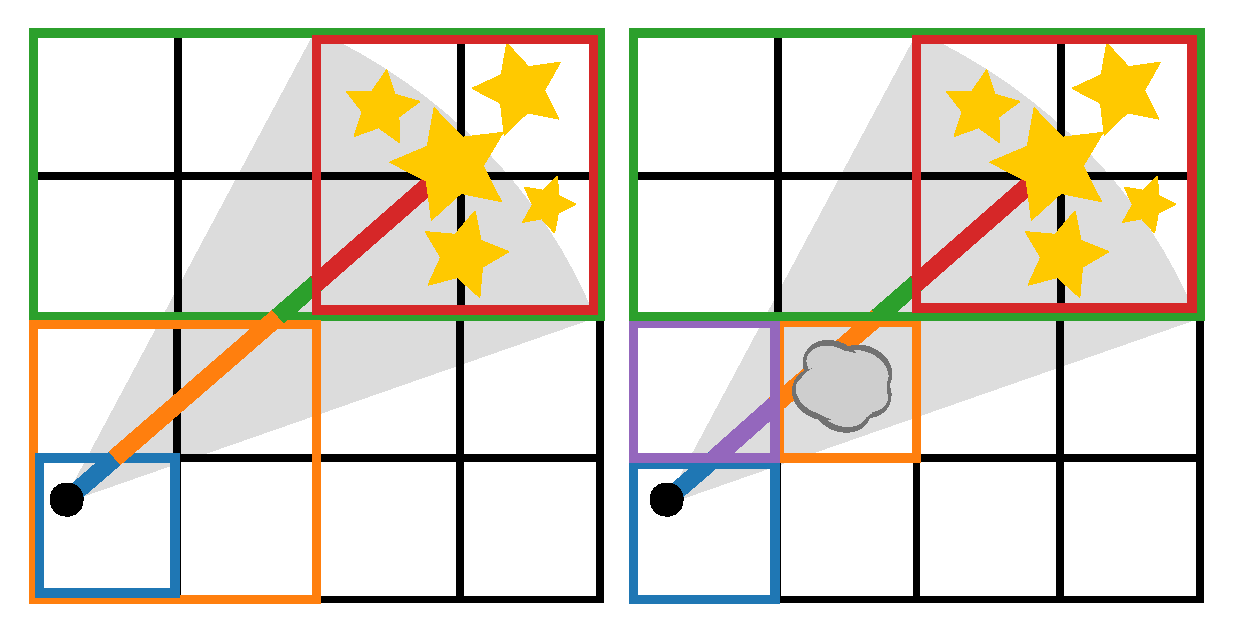
\includegraphics[width=1\linewidth]{Figures/algorithm.pdf}
\caption{}
\label{fig:algorithm}
\end{figure*}
The \acro{} algorithm is based around a tree data structure which partitions 
the simulation volume hierarchically in space. The smallest resolution 
elements, SPH gas particles in our case, live in the leaf nodes of the tree
data structure. The maximum number of resolution elements per leaf node or 
``bucket'' is a fixed parameter that is set to 10 for all runs in this 
paper. $N$ resolution elements hold radiation intensity values and 
represent the radiation field \acro{} computes. 

\subsubsection{Source Merging}
As mentioned in the introduction, a naive algorithm would compute interactions 
between a resolution element and  all sources of radiation (SPH star particles 
in our case). If we assume the number of resolution elements is equal to the 
number of sources, an infeasible number of interactions would need to be 
computed, scaling like $\bigO{N^2}$. To mitigate this $N^2$ scaling \acro{} 
employs source merging similar to particle merging in the \cite{barnesHut86} 
tree-based gravity solver which has remained common place in astrophysical 
simulations \citep{benz88,vineSigurdsson98,springelEt01,wadsleyEt03,
hubberEt11}. Sources of radiation are merged together at their centre of 
luminosity if they meet an ``opening angle'' criteria. This criteria is 
defined as 
\begin{equation}
\label{eq:openangle}
\theta_{\rm open} > l/s,
\end{equation}
where $l$ is the side length of a tree cell, $r$ is the distance between the 
centre of luminosity of a source and centre of mass of a resolution element 
and $\theta_{\rm open}$ is the opening angle, a fixed accuracy parameter. If a 
group of sources occupy the biggest tree cell that meets this criteria, all 
sources in that cell are merged into one, considerably reducing the number of 
interactions \acro{} computes. This is illustrated in the left panel of Fig. 
\ref{fig:algorithm}, where the grey angle represents a cell whose angular size 
meets the opening angle criterion.

The cost savings of source merging can be quantified by integrating to compute 
the number of tree cells that are ``opened'' according to the opening angle 
criteria. These opened cells will have their sources merged making them a 
count of $\NS$. We can do this by integrating spherical shells 
of thickness $dr$ along the distance from a resolution element $r$, and then 
dividing the sphere volume by the volume of an opened cell, $V_{\rm cell}(r)$.
\begin{equation}
\label{eq:nsint}
\NS = \int_{R_0}^R \frac{4\pi r^2}{V_{\rm cell}(r)} dr
\end{equation}
The bounds of the above integral go from $R_0$, the length of a bucket 
cell, to $R$, the length of the simulation volume. Because the number of 
particles in a simulation is proportional to the simulation volume, the 
lower integration limit can be expressed using particle numbers via 
\begin{equation}
\label{eq:ratio}
\frac{R_0}{R} = \sqrt[3]{\frac{N_B}{N}},
\end{equation} 
the cubed root of the ratio of the average number of particles per bucket, 
$N_B$, to the total number of simulation particles. The opened cell volume can 
also be rewritten by cubing the opening angle criteria
\begin{equation}
\label{eq:vcell}
V_{\rm cell}(r) = l^3 = \theta_{\rm open}^3 r^3.
\end{equation}
Substituting gives us the following integral and its solution,
\begin{equation}
\label{eq:nssoln}
\NS = \int_{\left(\frac{N}{N_B}\right)^{-\frac{1}{3}}}^R 
\frac{4\pi r^2}{\theta_{\rm open}^3} dr
\propto \log{N/N_B}.
\end{equation}
This results means that the number of interactions scales like 
$\bigO{N \log N}$. This is also the total cost scaling in the optically 
thin regime, which is unsurprising given the RT problem is almost identical to 
the gravity problem in the absence of intervening material. That brings up the 
next part of the algorithm, what to do about tracing a ray in the optically 
thick regime.

\subsubsection{Tracing Rays}
In the presence of absorbing material along a ray, the optical depth needs to 
be computed along said ray by computing the optical depth integral introduced 
in Eq. \ref{eq:tauint}. To solve this integral numerically, we traverse the 
tree between the interacting source and resolution element to build up the 
optical depth. This is possible because the tree is partitioned in and fills 
space, thus all the intervening material should be contained in the sub-tree 
we traverse. Making use of properties computed during the tree build, we can 
compute the optical depth of a piece of the ray using the geometry of the cell 
and ray as well as the average density and opacity in the cell
\begin{equation}
\label{eq:taui}
\tau_i = \bar{\rho}_i \bar{\kappa}_i s_i.
\end{equation}
The total optical depth is then summed up during the tree walk,
\begin{equation}
\label{eq:tausum}
\tau = \sum_i \tau_i,
\end{equation}
giving us everything needed to evaluate Eq. \ref{eq:simpflux}. This process 
is also illustrated in the left panel of Fig. \ref{fig:algorithm}, where there 
are two important things to note. Firstly, since we are performing a reverse 
ray trace similar to that of URCHIN \citep{altayTheuns13}, the resolution 
element denoted by the black circle is intrinsically well resolved at the 
bucket cell (denoted by the blue cell) level. However, the second point is 
that as the tree is walked upwards space becomes less resolved. In Fig. 
\ref{fig:algorithm} the colour of highlighted cells corresponds to which 
pieces of the ray their properties are used to compute. It should be apparent 
that the central parts of the ray are less resolved (the green cell) and as 
you move towards the source or resolution element the ray becomes more 
resolved (the red and orange cells). This can be looked at in two ways. 
If the medium is uniform, the algorithm can be extremely efficient 
while still being able to resolve a sharp feature in the radiation field such 
as an ionization front. However, if the medium is highly irregular along the 
ray the algorithm will not be to resolve sharp density distributions which 
could significantly alter the optical depth. Adaptive refinement is needed 
during the tree walk to accurately resolve the medium along the ray.

\subsubsection{Adaptive Refinement}
Consider the right panel in Fig. \ref{fig:algorithm}. A dense blob of gas 
to be resolved resides in the orange highlighted cell. At the point in the 
tree walk where we reach the orange highlighted cell in the left panel, a 
decision needs to be made on whether the current cell sufficiently represents 
the media. This decision is made by a refinement criteria. If the cell passes 
the criteria to refine, rather than using its average properties we 
recursively check the cell's children until the criteria fails. Thus building 
a better resolved section of the ray. 

Difficulty comes in choosing a refinement criteria that is both accurate and 
efficient. Ideally, the criteria should be true when an average optical depth 
in a region may not be accurate to the true distribution, such as a clumpy 
medium where the average density and opacity is much higher than the 
``effective'' density and opacity \citep{varosiDwek99, hegmanKegel03}. For 
this reason we have chosen optical depth to be the basis of our refinement 
criteria.

\begin{figure}
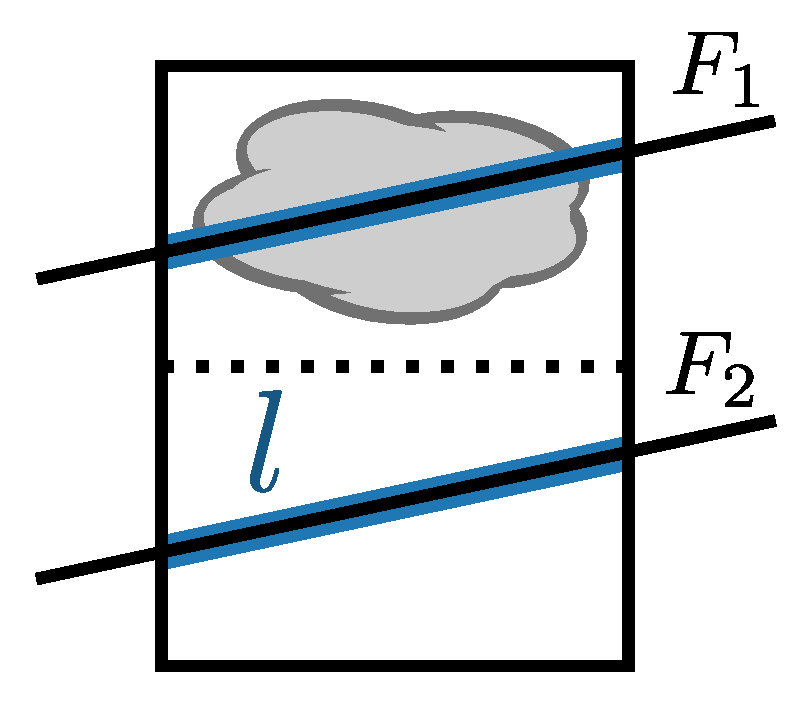
\includegraphics[width=1\linewidth]{Figures/refine.pdf}
\caption{}
\label{fig:refine}
\end{figure}
Our optical depth based refinement criteria is unique to \acro. Consider two 
rays through through a large cell as in Fig. \ref{fig:refine} (note that his 
description is simplified to 2D). These rays represent what the case would be 
if properties of the children were used instead of the parent cell. We can 
compute the minimum and maximum absorption coefficients $\alpha_{\rm min}$ and 
$\alpha_{\rm max}$, via their average density and opacity values computed 
during the tree build. This multiplied by the intersection length $l$ gives us 
the minimum and maximum optical depths, $\tau_{\rm min}$ and $\tau_{\rm max}$. 
We can then test the following refinement criteria
\begin{equation}
\label{eq:refcrit}
\tau_{\rm refine} < \tau_{\rm max} - \tau_{\rm min},
\end{equation}
and refine if it is true. The fractional error in flux for a chosen value of 
$\tau_{\rm refine}$ is
\begin{equation}
\label{eq:reffrac}
\frac{F_1 - F_2}{F_1} \leq 1 - e^{-\tau_{\rm max}-\tau_{\rm max}} 
< \tau_{\rm refine},
\end{equation}
for small $tau$, making the refinement criteria a convenient choice of 
parameter for guaranteeing accuracy.

If the refinement criteria passes at the bucket level, individual particles 
within a bucket are considered. An straight forward $N^2$ ray tracing scheme 
similar to SPHRay \citep{altayEt08} can be performed. This should contribute 
negligible cost to the algorithm as the number of particles in a bucket is 
less than 10.

Fully characterizing the computational cost of the algorithm including the 
addition of adaptive refinement follows the same method as used earlier. 
However, now instead of integrating the number of sources we integrate the 
total number of ray segments computed. We will look at two cases, not refining 
at all and fully refining down to the bucket level. This will give us upper 
and lower bound for the algorithms scaling as characterizing the refinement 
between these extremes depends on the specific density and opacity 
distributions being operated on.

First let's consider the case where the refinement criteria always passes and 
all rays are resolved down to the bucket level. The number of segments per ray 
is then just the length of a ray divided by the size of a bucket. We can 
express this as
\begin{equation}
\label{eq:nseg}
N_{\rm seg} = \frac{r}{R_0} = \frac{r}{R}\left(\frac{N}{N_B}\right)^\frac{1}{3}
\end{equation}
after substituting Eq. \ref{eq:ratio} in for $R_0$. Since $\NS$ is also the 
number of rays computed, the total number of ray segments computed is just Eq. 
\ref{eq:nsint} multiplied by the number of ray segments
\begin{equation}
\label{eq:nsegint}
N_{\rm seg} = \int_{\left(\frac{N}{N_B}\right)^{-\frac{1}{3}}}^R 
\frac{4\pi r^2}{\theta_{\rm open}^3}
\frac{r}{R}\left(\frac{N}{N_B}\right)^\frac{1}{3} dr
\propto N(2N/N_B)^\frac{1}{3}.
\end{equation}
This results means that the total cost of the algorithm scales like 
$\bigO{N^{4/3}}$ in the worst case.

In the case were the refinement criteria never passes, the ray is split into 
segments made up of the cells traversed in the tree walk of the sub-tree going 
from source to resolution element. The number of cells traversed in a tree walk
is equal to the logarithm of the number of leaf nodes contained within the 
sub-tree. The number of leaf nodes in the sub-tree is also given by Eq. 
\ref{eq:nseg}, so by taking the logarithm of Eq.\ref{eq:nseg} and adding two 
for the two buckets on eiter side of the sub-tree we come to
\begin{equation}
\label{eq:nseg2}
N_{\rm seg} = \log_2\left[\frac{r}{R}\left(
\frac{N}{N_B}\right)^\frac{1}{3}\right],
\end{equation}
where the logarithm is base two as \acro{} is implemented with a binary tree. 
Like before we multiply Eq. \ref{eq:nsint} by the number of ray segments and 
integrate the following
\begin{equation}
\label{eq:nsegint2}
N_{\rm seg} = \int_{\left(\frac{N}{N_B}\right)^{-\frac{1}{3}}}^R 
\frac{4\pi r^2}{\theta_{\rm open}^3}
\log_2\left[\frac{r}{R}\left(
\frac{N}{N_B}\right)^\frac{1}{3}\right] dr
\propto N\log^2(128 N/N_B).
\end{equation}
This results means that the total cost of the algorithm scales like 
$\bigO{N\log^2N}$ in the best case.

\subsection{Cosmological Background Radiation}
\begin{figure}
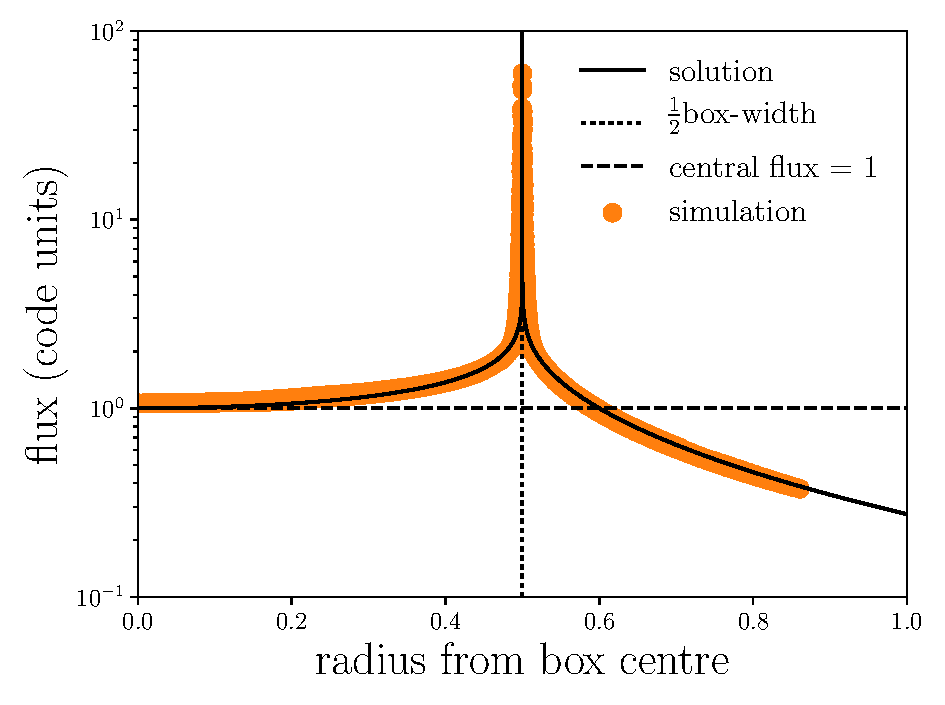
\includegraphics[width=1\linewidth]{Figures/cosmofield.pdf}
\caption{}
\label{fig:cosmof}
\end{figure}
In order to treat cosmological simulations properly we must account for the 
radiation coming from the rest of the universe outside of the simulation 
volume. Most current codes apply a constant UV field to the entire box, 
essentially the lowest order approximation possible. Some specialized codes 
like URCHIN {altayTheuns13} do a reverse ray trace to the edge of the 
box, where the background flux is assumed to be coming from. Others, such as 
TRAPHIC {pawlikSchaye08} allow their ray trace to be periodic. We believe
that this periodic treatment is problematic for reasons we will explain at the
end of this subsection (well... we haven't figured it out yet). 

Instead, we have implemented a method involving ``background sources''. 
``Background'' particles are distributed in a spiral pattern on the surface of 
a sphere at the very edge of the simulation volume (or at a large distance if 
required) and the number of sources can be varied to match the required 
angular resolution  of the background. Finding the flux at the centre of a 
sphere of sources is a problem akin to Newton's Shell Theorem. However, 
because the intensity does not cancel like force, the solution differs and is 
as follows:
\begin{equation}
\label{eq:cosmof}
F(r) = \frac{L}{8\pi R} \ln \left(\frac{R+r}{R-r}\right),
\end{equation}
where $L$ is the total luminosity of the emitting shell, $R$ is the radius of 
the sphere and $r$ is the radius the flux is being computed at. The shape of 
the function can be seen in Figure \ref{fig:cosmof} where we have plotted the 
flux as a function of radius for a homogeneous, optically thin test volume.

Note that due to the logarithm in equation \ref{eq:cosmof}, the flux is nearly 
constant at small radii. Since most cosmological zoom in simulations only 
consider gas at a fairly small radius, this setup of background sources is an 
acceptable method to provide a cosmological background flux. A benefit of this 
method is that we can use all of the existing machinery described in the 
methods section, and only have to add temporary background star particles as 
the source of the background radiation. This way, there is no need to create 
periodic copies of the simulation volume (talk to James, explain <-this here).





\section{CODE TESTS}\label{sec:tsts}
\subsection{Scaling with number of resolution elements}
\begin{figure}
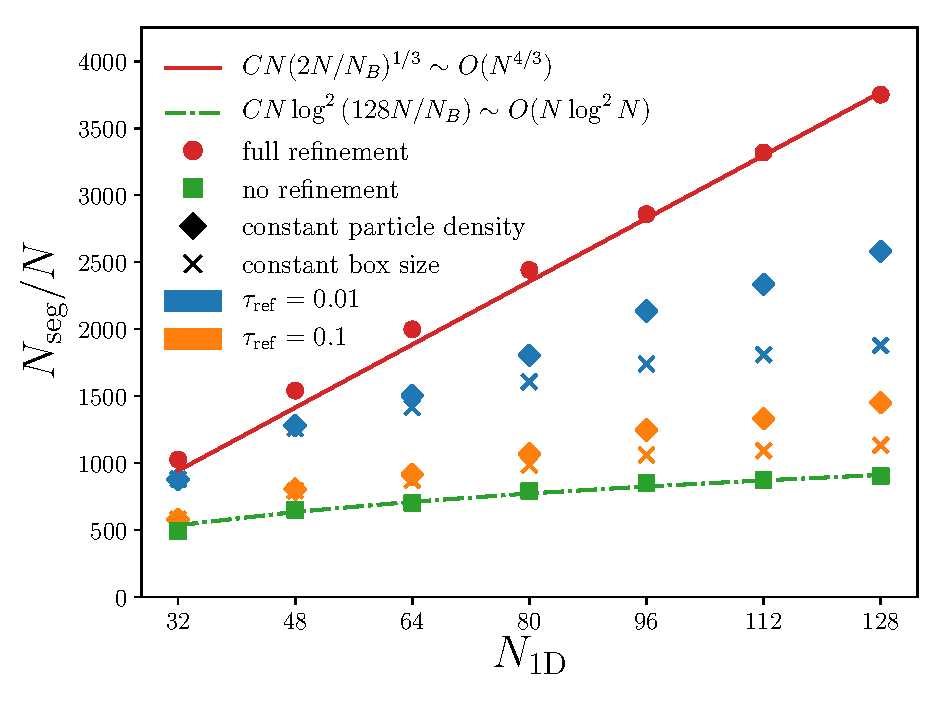
\includegraphics[width=1\linewidth]{Figures/particle_scaling.pdf}
\caption{}
\label{fig:pscale}
\end{figure}
\subsection{Opening Angle Testing}
\begin{figure}
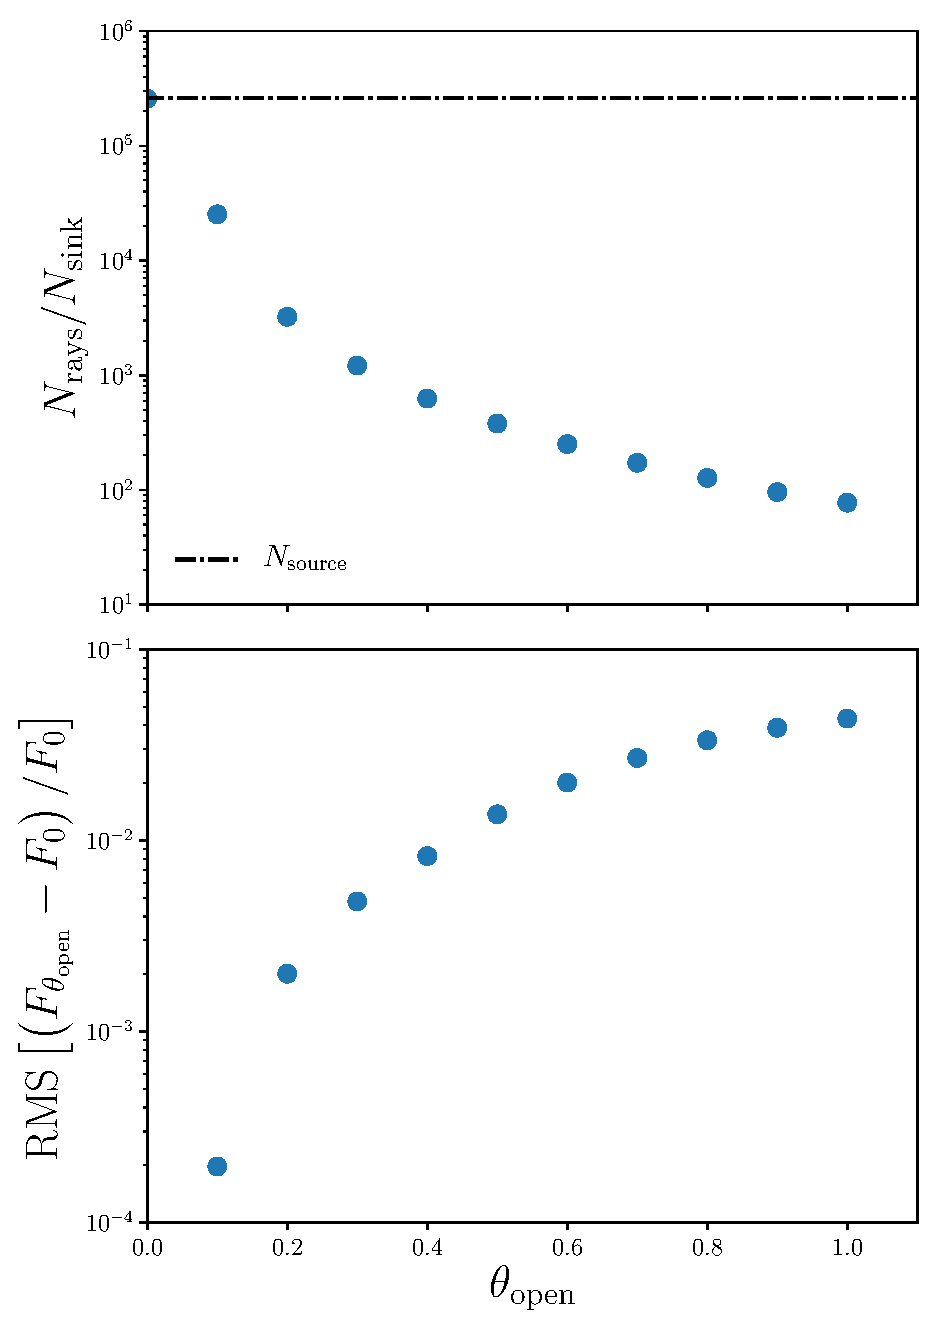
\includegraphics[width=1\linewidth]{Figures/opening_angle.pdf}
\caption{}
\label{fig:openangle}
\end{figure}
\subsection{Refinement Criteria Testing}
\begin{figure}
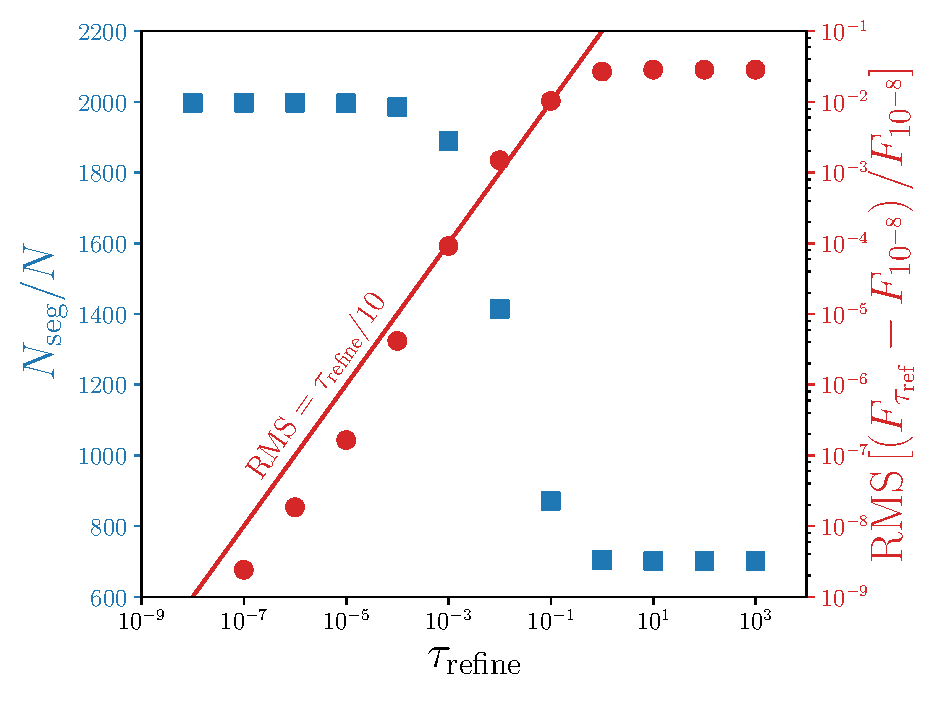
\includegraphics[width=1\linewidth]{Figures/refinement_criteria.pdf}
\caption{}
\label{fig:refcrit}
\end{figure}
\subsection{Isothermal Spheres}
\begin{figure}
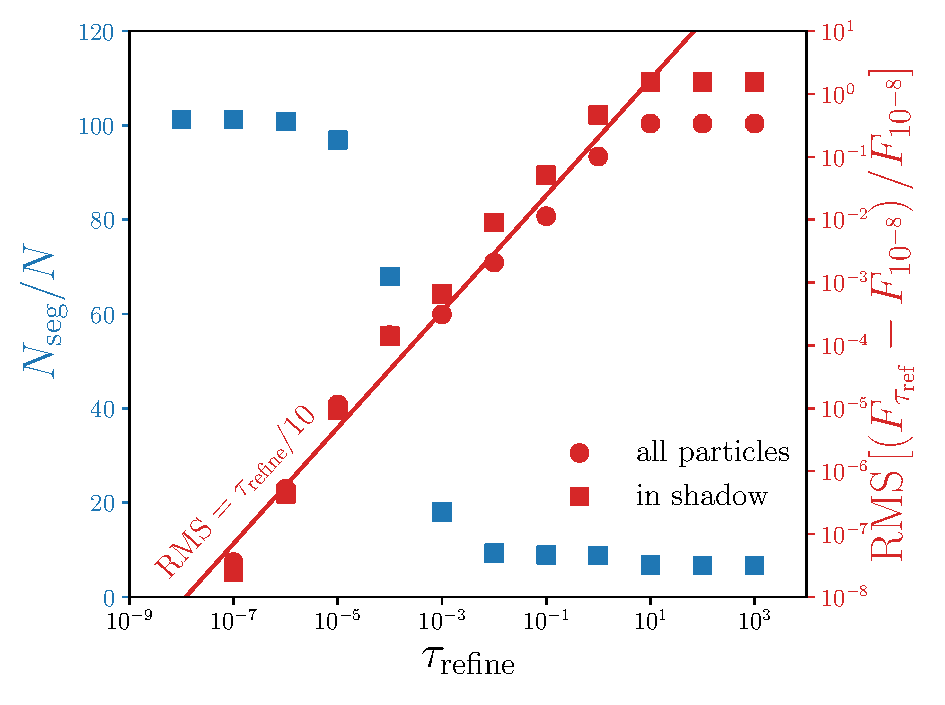
\includegraphics[width=1\linewidth]{Figures/isothermal_spheres.pdf}
\caption{}
\label{fig:isosph}
\end{figure}
\subsection{Str\"{o}mgren Sphere Test}
\begin{figure*}
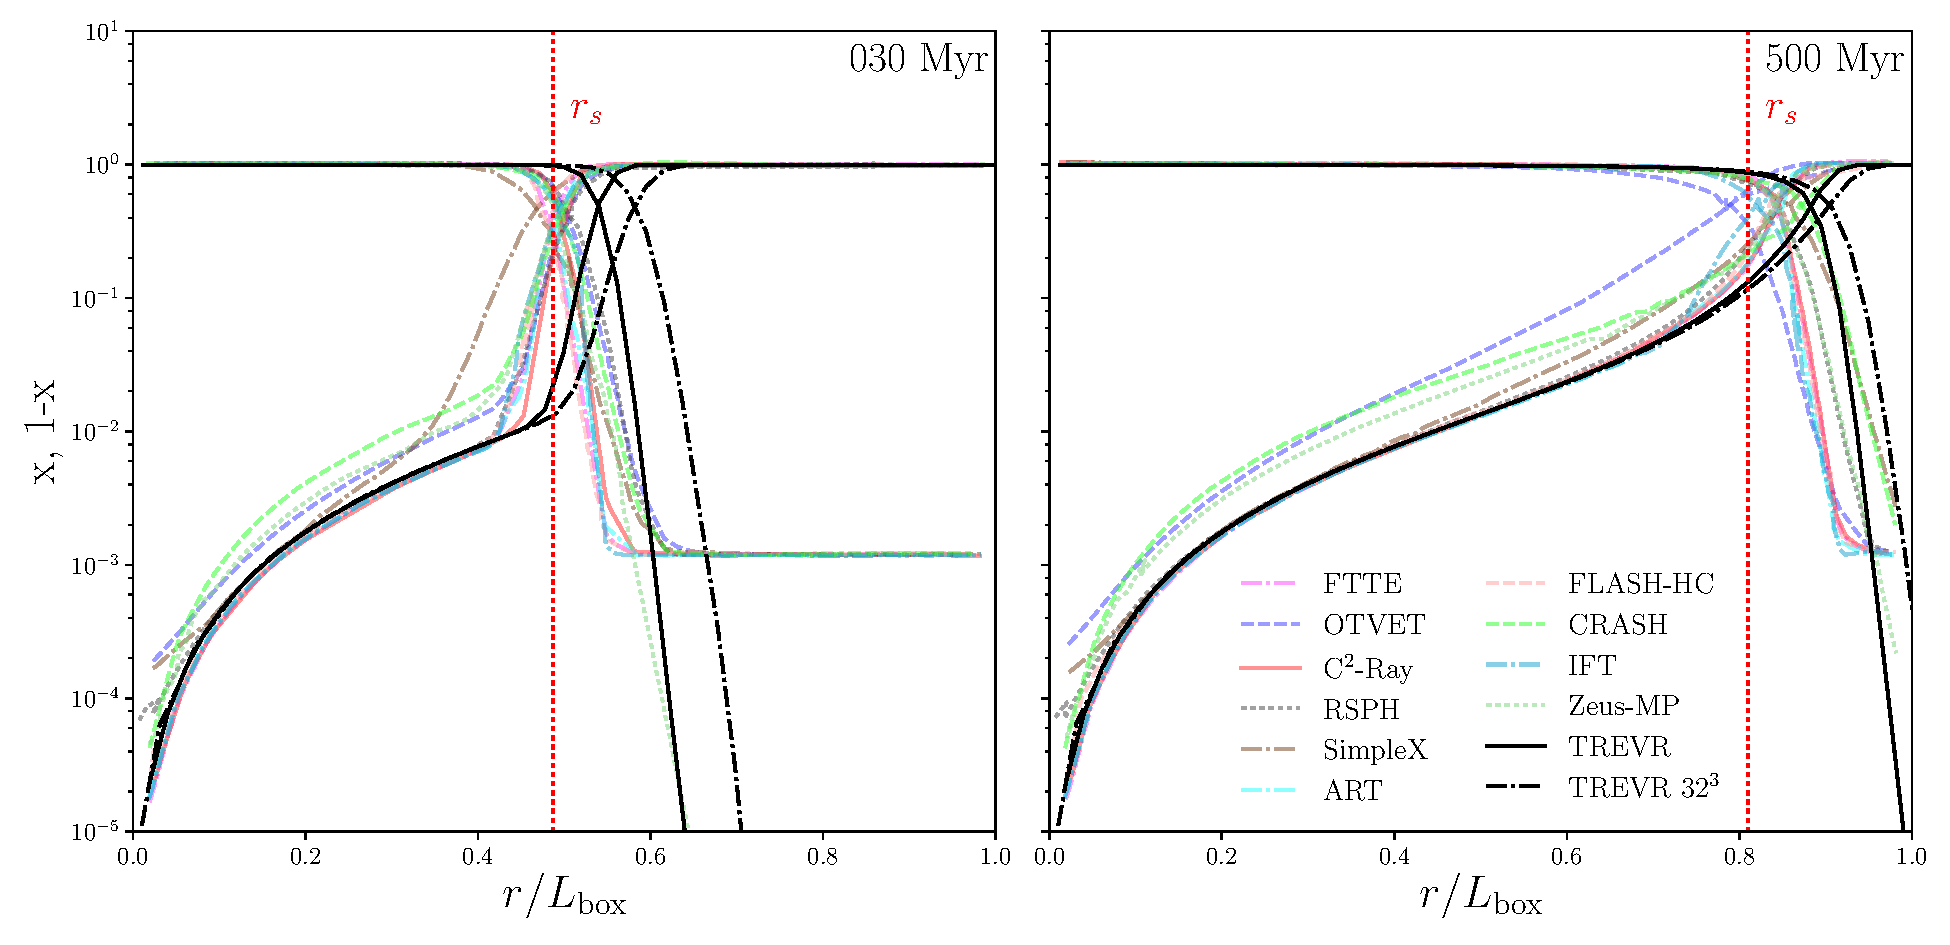
\includegraphics[width=1\linewidth]{Figures/strom_iso_fraction.pdf}
\caption{}
\label{fig:stromiso}
\end{figure*}
\begin{figure*}
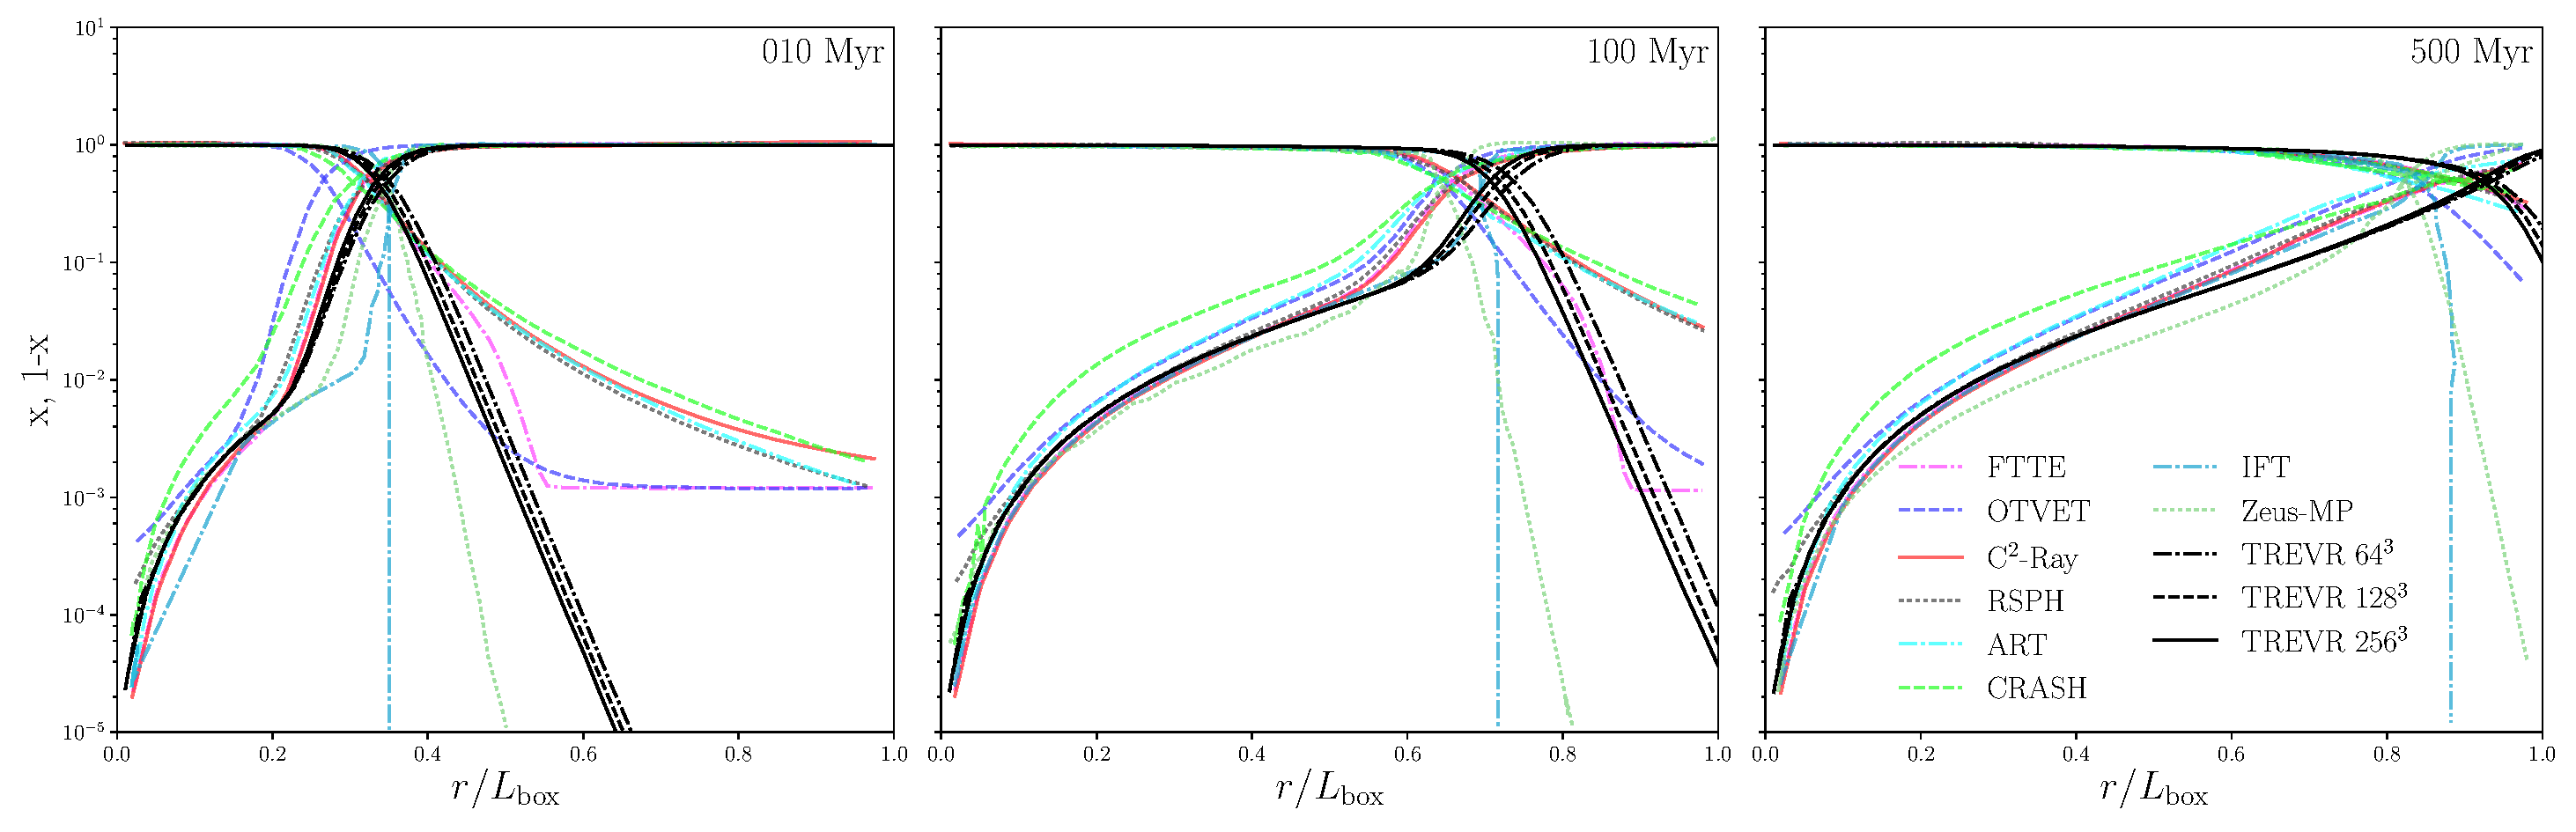
\includegraphics[width=1\linewidth]{Figures/strom_fraction.pdf}
\caption{}
\label{fig:stromtherm}
\end{figure*}
\begin{figure*}
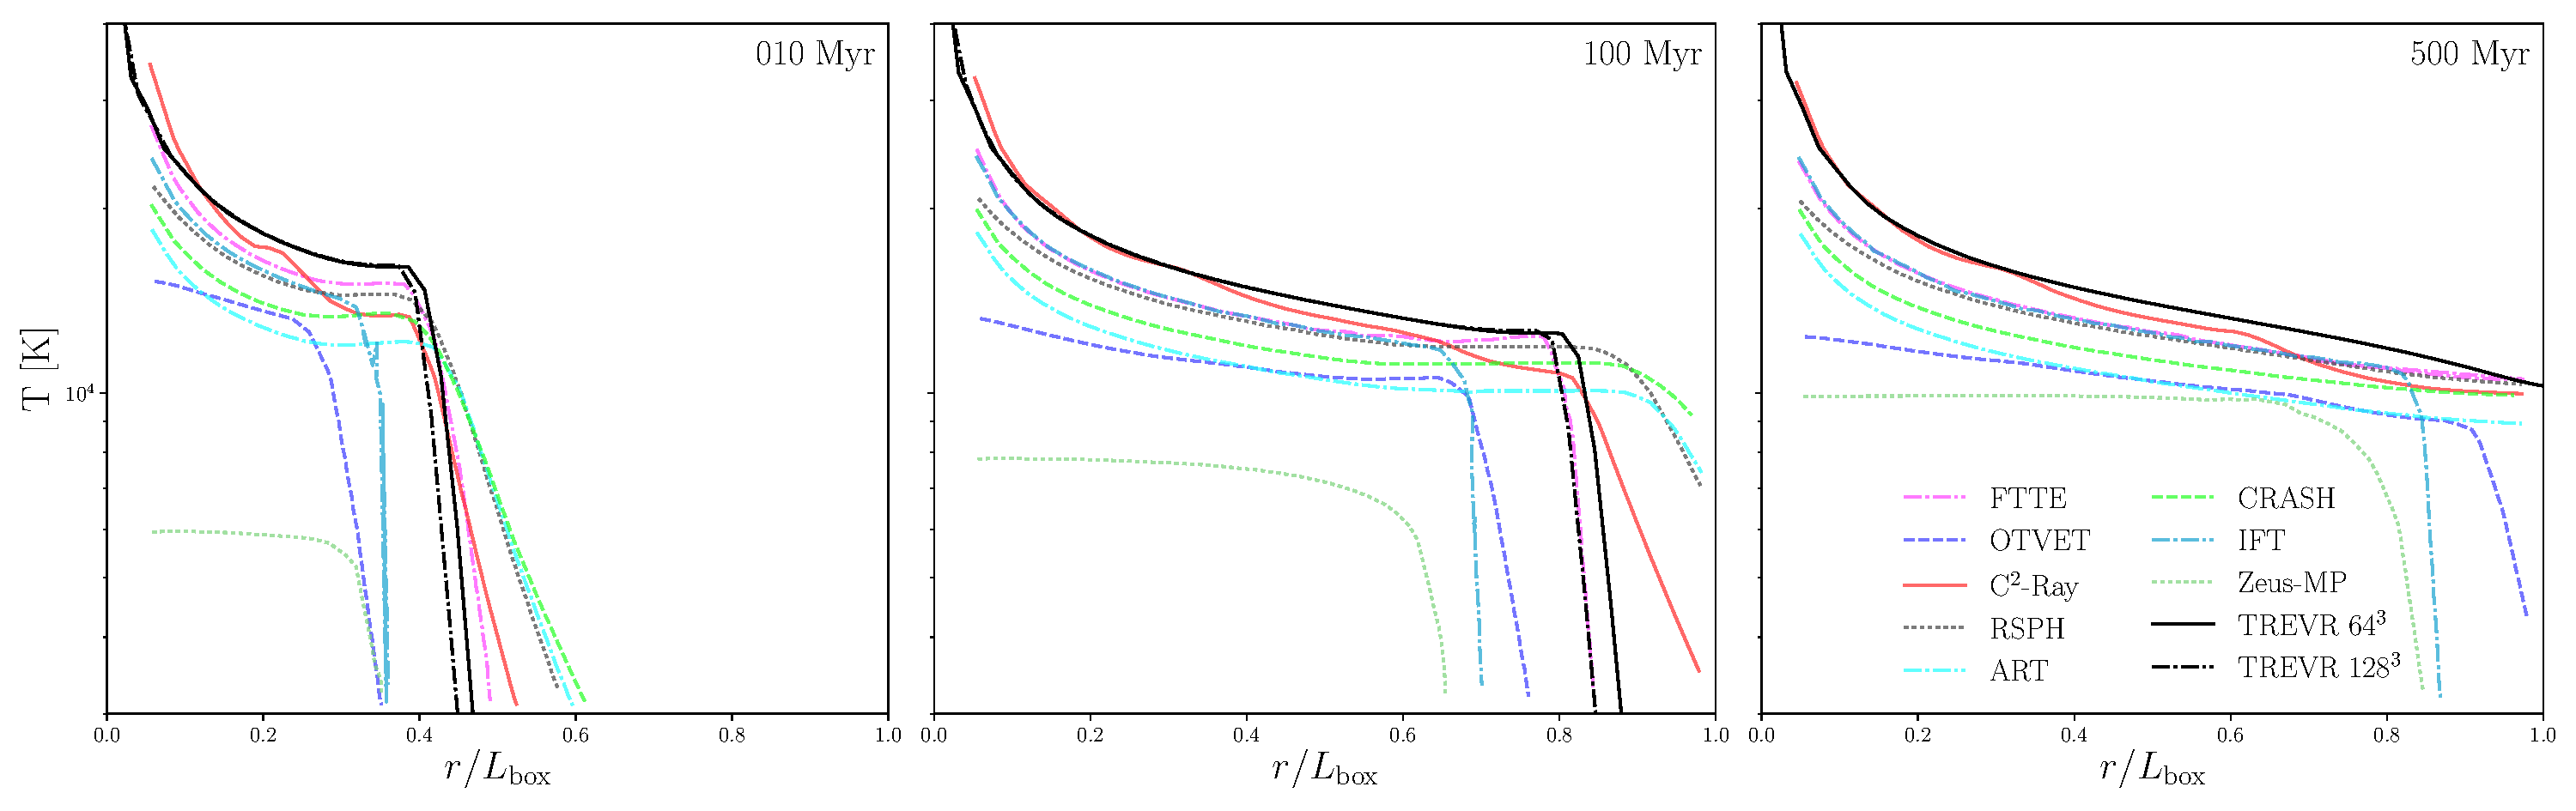
\includegraphics[width=1\linewidth]{Figures/strom_temp.pdf}
\caption{}
\label{fig:stromtemp}
\end{figure*}
\section{DISCUSSION AND CONCLUSION}\label{sec:disc}

\section*{Acknowledgements}\label{sec:ackn}

%%%%%%%%%%%%%%%%%%%%%%%%%%%%%%

%%%%%%%%%% REFERENCES %%%%%%%%%%

\bibliographystyle{mnras}
\bibliography{references}

%%%%%%%%%%%%%%%%%%%%%%%%%%%%%%

%%%%%%%%%% APPENDICES %%%%%%%%%%

\appendix
\section{Test Initial Conditions}\label{sec:icnd}
%%%%%%%%%%%%%%%%%%%%%%%%%%%%%%

\bsp
\label{lastpage}
\end{document}

%%%%%%%%%% FIN %%%%%%%%%%
